\documentclass[a4paper, twocolumn]{article}
\newcommand{\spc}{\vspace{5mm}}

\usepackage[utf8]{inputenc}
\usepackage[T1]{fontenc}
\usepackage[spanish]{babel}

\usepackage{amsmath}
\usepackage{graphicx}
\usepackage{hyperref}
\usepackage{amssymb}
\usepackage{color}
\usepackage{listings}
\usepackage{times}

\graphicspath{ {images/} }


\begin{document}

\title{Formulario Finanzas}
\author{Sebastián Lévano}
\date{\today}
\maketitle

% \section{Tiempo}

% \begin{figure}
%     \centering
%     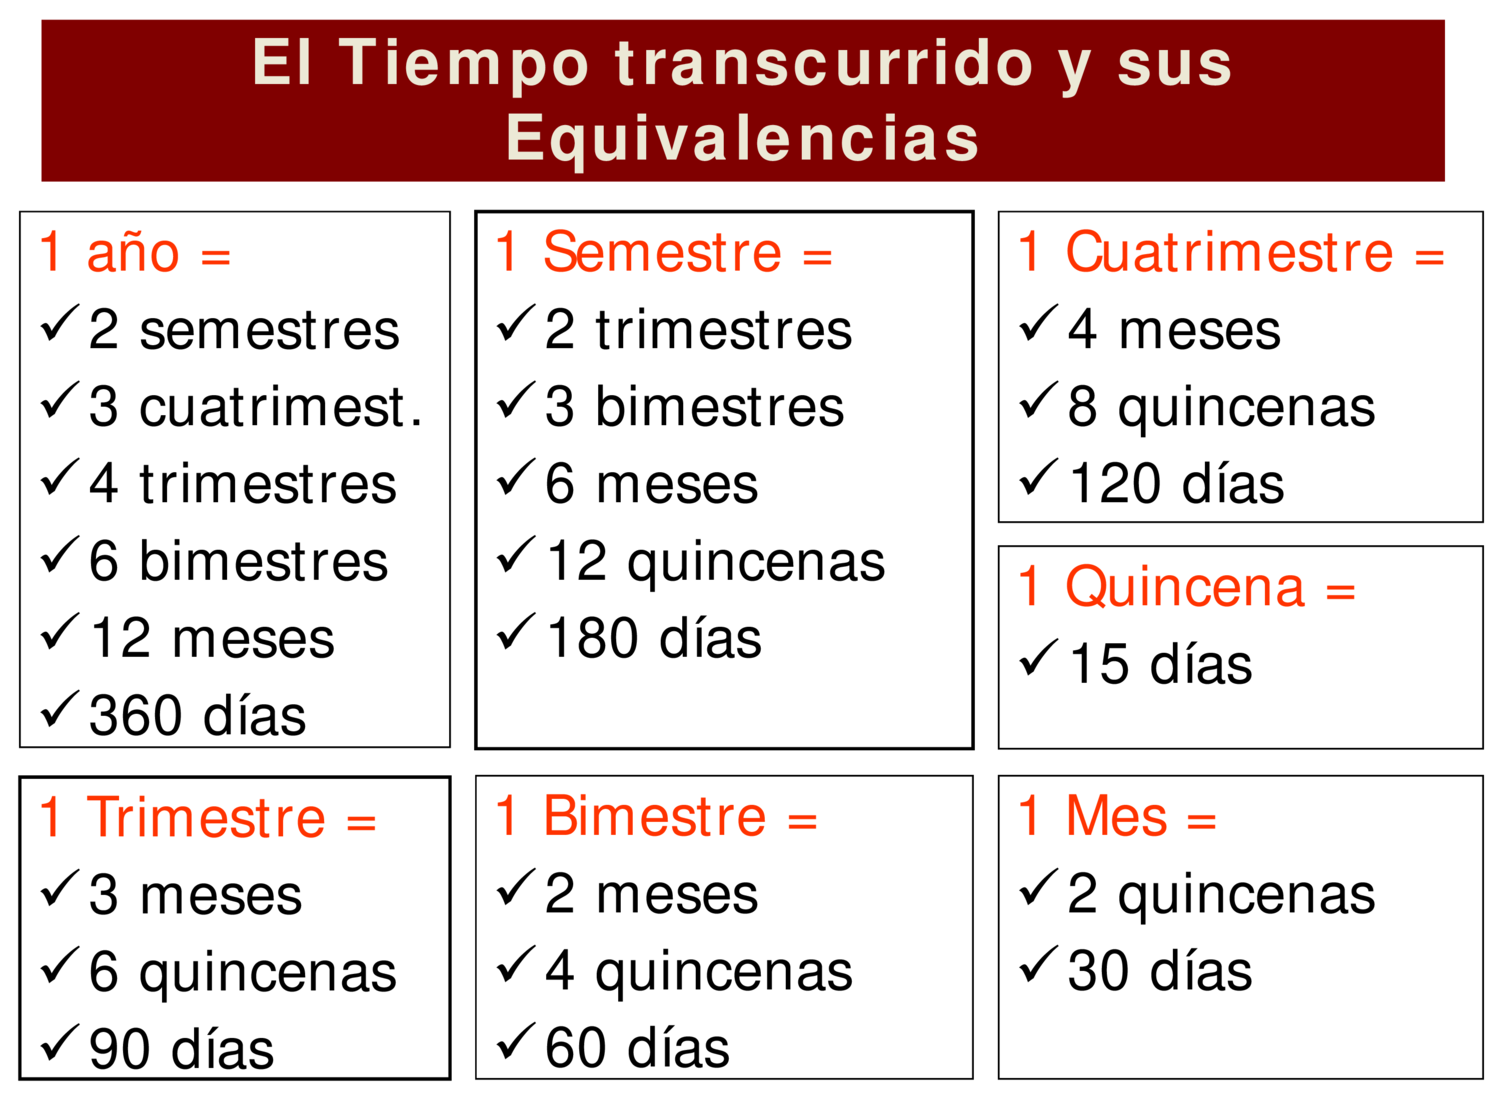
\includegraphics[scale=0.33]{Tiempo_Equivalencias}
% \end{figure}

% \begin{figure}
%     \centering
%     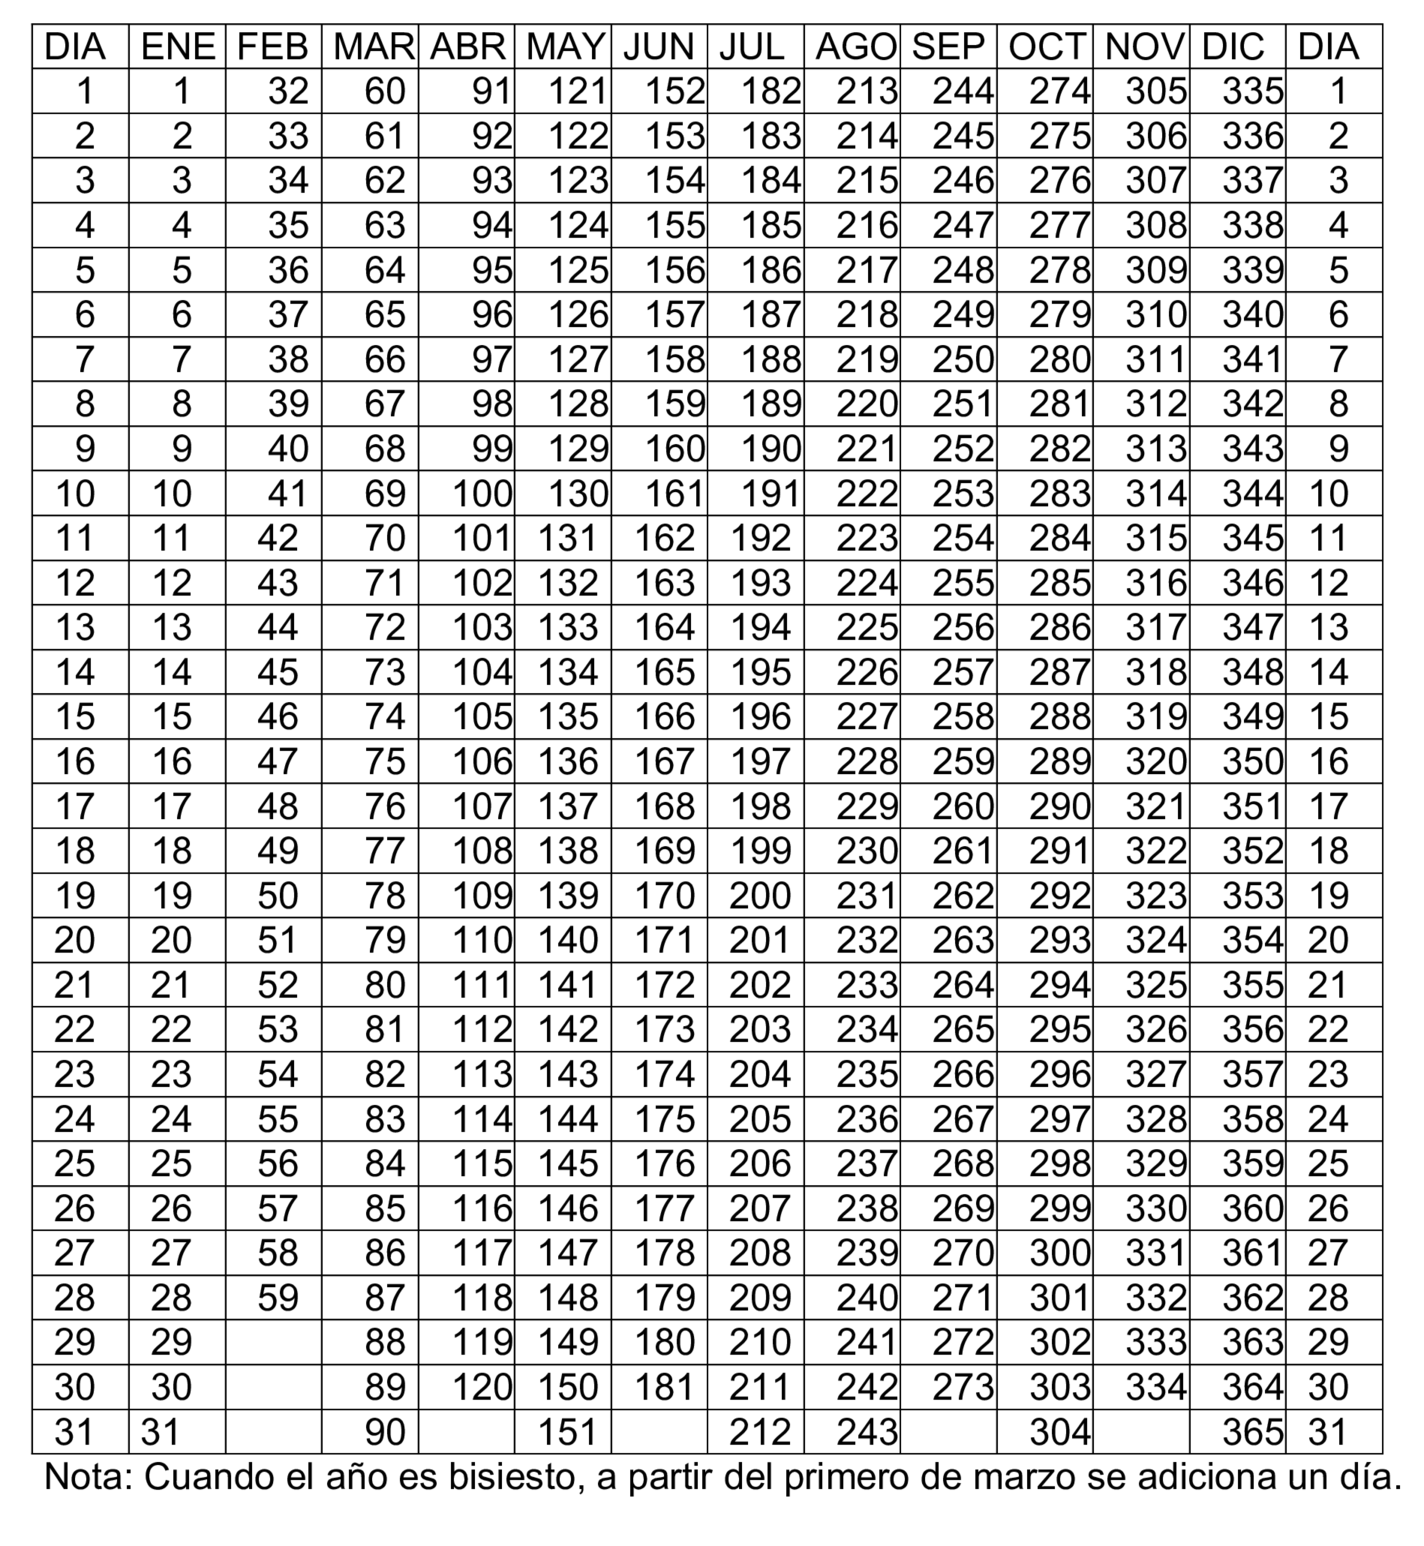
\includegraphics[scale=0.35]{Tabla_Dias}
% \end{figure}

\section{Interés Simple}

\begin{gather*}
    I = S - C \\
    I = C \cdot i \cdot t \\
    S = C \cdot (1 + i \cdot t) \\
    C = \frac{S}{(1 + i \cdot t)} \\
    C = S \cdot (1 + i \cdot t)^{-1} \\
    D = d \% C \\
    i = \frac{(\frac{S}{C} - 1)}{t} \cdot 100 \% \\
    Saldo = C - D \\
    P_l = P_c + recargo \% \cdot P_c \\
    C = P_c - C_i \\
    S = P_l - C_i
\end{gather*}

Donde:

\begin{align*}
    I = \text{Interés}                                \\
    S = \text{Stock - Monto - Valor Futuro}           \\
    C = \text{Capital - Valor Presente}               \\
    i = \text{Tasa de interés}                        \\
    t = \text{Tiempo}                                 \\
    (1 + i \cdot t) = \text{Factor de acumulación}    \\
    \text{a tasa de interés simple}                   \\
    (1 + i \cdot t)^{-1} = \text{Factor de descuento} \\
    \text{a tasa de interés simple}                   \\
    P_l = \text{Precio de lista}                      \\
    P_c = \text{Precio de venta - Precio al contado}  \\
\end{align*}


\section{Interés Nominal}


\begin{gather*}
    i' = \frac{TN}{m} \\
    TEP = (\frac{S}{C} - 1) \cdot 100 \% \\
    S = C \cdot (1 + i')^n \\
    S = C \cdot (1 + \frac{TN}{m})^n \\
    C = \frac{S}{(1 + \frac{TN}{m})^n} \\
    C = S \cdot {(1 + \frac{TN}{m})^{-n}} \\
    n = \frac{\ln{\frac{S}{C}}}{\ln{(1 + \frac{TN}{m})}} \\
    TN = m \cdot (\sqrt[n]{\frac{S}{C}} - 1) \cdot 100 \% \\
\end{gather*}

Donde:

\begin{align*}
    I = \text{Interés}                                \\
    S = \text{Stock - Monto - Valor Futuro}           \\
    C = \text{Capital inicial - Valor Presente}       \\
    i' = \text{Tasa de interés}                       \\
    \text{en el periodo de capitalización}            \\
    TN = \text{Tasa nominal}                          \\
    TEP = \text{Tasa efectiva anual}                  \\
    t = \text{Tiempo}                                 \\
    n = \text{Número de periodos}                     \\
    m = \text{Número de veces}                        \\
    \text{que se repite el periodo de capitalización} \\
\end{align*}

\subsection{Recordatorios}

\begin{itemize}
    \item Todos los tiempos se rigen por la capitalización.
    \item La $TEP$ se haya en abse al tiempo.
          Ejemplo: $t = 6$ meses, entonces se haya una $TES$
\end{itemize}

\section{Interés Efectivo}

\begin{gather*}
    TEP = (\frac{S}{C} - 1) \cdot 100 \% \\
    TEP = ((1 + \frac{TN}{m})^n - 1) \cdot 100 \% \\
    TN = m \cdot (\sqrt[n]{1 + TEP} - 1) \cdot 100 \% \\
    TEP_2 = (1 + TEP_1)^{\frac{n_2}{n_1}} - 1) \cdot 100 \% \\
    S = C \cdot (1 + TEP)^n \\
    S = C \cdot (1 + TEP)^{\frac{\text{Nro días trasladar}}{\text{Nro días TEP}}} \\
    C = \frac{S}{(1 + TEP)^{\frac{\text{Nro días trasladar}}{\text{Nro días TEP}}}} \\
    n = \frac{ln{\frac{S}{C}}}{ln{1 + TEP}} \cdot {\text{Nro días TEP}} \\
    TEP = (\frac{S}{C})^{\frac{\text{Nro días TEP}}{\text{Nro días trasladar}}} - 1 \\
\end{gather*}

Donde:

\begin{gather*}
    m = \text{Número de capitalizaciones de la Tasa Nominal} \\
    \text{en el tiempo que quedo expresada} \\
    n = \text{Número de capitalizaciones realizadas} \\
    \text{en el tiempo de la inversión} \\
\end{gather*}

\section{Tasa Descontada}

\begin{gather*}
    \text{Descuento} = \text{Valor Nominal} \cdot d\% \\
    \text{Valor Neto} = \text{Valor Nominal} - \text{Descuento} \\
    \text{Valor Neto} = \text{Valor Nominal} \cdot (1 - d\%) \\
    d\% = \frac{i'}{1 + i'} \\
    i' = \frac{d\%}{1 - d\%} \\
    \text{Valor Neto} = \text{Valor Nominal} \cdot (1 + TE)^{\frac{nd}{n}} \\
    TEtd = (1 + \frac{TN}{m})^n - 1 \\
    TEtd = (1 + TEP)^\frac{td}{n} - 1 \\
    dt = \frac{TEtd}{1 + TEtd} \\
    d\% = dt \\
    \text{Valor recibido} = \text{Valor Neto} - \text{Suma de los costes} \\
    \text{iniciales} - \text{Retención} \\
    \text{Valor entregar / cancelar} = \text{Valor Nominal} + \text{Suma de} \\
    \text{los costes finales} - \text{Retención} \\
    TCEA = \frac{\text{Valor Entregado}}{\text{Valor Recibido}}^\frac{360}{td} - 1 \\
    Ic = \text{Valor Nominal} \cdot [(1 + TEP1)^\frac{td}{n1} - 1] \\
    Ic = \text{Valor Nominal} \cdot [(1 + \frac{TN}{m})^n - 1] \\
    Im = \text{Valor Nominal} \cdot [(1 + TEPmora)^\frac{td}{n1} - 1] \\
    Im = \text{Valor Nominal} \cdot [(1 + \frac{TN}{m})^n - 1] \\
    \text{Valor Entregado} = \text{Valor Nominal} + \\
    \text{Suma de Costes Finales} - \text{Retención} + \\
    \text{Interés compensatorio} + \text{Interés moratorio} + \\
    \text{Suma de Costes por la mora} \\
    TCEAm = (\frac{\text{Valor entregado mora}}{\text{Valor Recibido}})^{\frac{360}{td + tm}} - 1 \\
\end{gather*}

\newpage

Donde:

\begin{gather*}
    i' = \text{Tasa Efectiva en el Período de descuento (TEP)} \\
    d\% = \text{Tasa de Descuento equivalente} \\
    nd = \text{Número de días de descuento} \\
    n = \text{Número de días del período de descuento} \\
    td = \text{Tiempo transcurrido desde la fecha del descuento} \\
    TEtd = \text{Tasa Efectiva en el período de tiempo} \\
    \text{transcurrido} \\
    TCEA = \text{Tasa de Coste Efectivo Anual} \\
    Ic = \text{Intereses compensatorios} \\
    In = \text{Intereses moratorios} \\
    TCEAm = \text{Tasa de Coste Efectivo Anual de la} \\
    \text{Operación incluyendo mora} \\
\end{gather*}

\section{Anualidades}

\subsection{Fórmula para anualidad simple vencida}

\begin{gather*}
    R = C \cdot (\frac{i \cdot (1 + i)^n}{(1 + i)^n - 1}) \\
    R = S \cdot (\frac{i}{(1 + i)^n - 1}) \\
\end{gather*}

\subsection{Fórmula para anualidad simple adelantada}

$$ Ra = C \cdot (\frac{i \cdot (1 + i)^{n - 1}}{(1 + i)^n - 1}) $$

\subsection{Factores financieros}

\subsubsection{Factor de capitalización de la serie (FCS)}

$$ FCS = [\frac{(1 + i)^n - 1}{i}] $$

\subsubsection{Factor de déposito al fondo de amortización (FDFA)}

$$ FDFA = \frac{i}{(1 + i)^n - 1} $$

\subsubsection{Factor de recuperación del capital (FRC)}

$$ FRC = [\frac{i \cdot (1 + i)^n}{(1 + i)^n - 1}] $$

\subsubsection{Factor de recuperación del capital (FAS)}

$$ FAS = [\frac{(1 + i)^n - 1}{i \cdot (1 + i)^n}] $$

\section{Indicadores de Rentabilidad}

\subsection{Valor Actual Neto (VAN)}

\begin{gather*}
    VA = \sum_{t = 1}^{n} \frac{FC_t}{(1 + COK)^t} \\
    VAN = - \text{Inversión} + VA \\
    VAN = - \text{Inversión} + \sum_{t = 1}^{n} \frac{FC_t}{(1 + COK)^t} \\
\end{gather*}

Donde:

\begin{gather*}
    VA = \text{Valor Actual} \\
    FC_t = \text{Flujo de Caja en el período t} \\
    COK = \text{Costo de Oportunidad del Capital} \\
    n = \text{Número de períodos} \\
\end{gather*}

\subsubsection{Criterios de Aceptación o Rechazo}

\begin{gather*}
    VAN > 0 \rightarrow \text{Aceptar} \\
    VAN < 0 \rightarrow \text{Rechazar} \\
    VAN = 0 \rightarrow \text{Indiferente} \\
\end{gather*}

\subsection{Tasa de Interna de Retorno (TIR)}

\subsubsection{Criterios}

\begin{gather*}
    TIR > COK \rightarrow \text{Vale la pena} \\
    TIR < COK \rightarrow \text{No vale la pena} \\
    TIR = COK \rightarrow \text{Indiferente} \\
\end{gather*}

\subsection{Índice Beneficio / Costo}

\begin{gather*}
    B / C = \frac{VA}{\text{Inversión}} \\
    B / C = \frac{\sum_{t = 1}^{n} \frac{FC_t}{(1 + COK)^t}}{\text{Inversión}} \\
\end{gather*}

\subsubsection{Criterios}

\begin{gather*}
    B / C > 1 \rightarrow \text{Aceptar} \\
    B / C < 1 \rightarrow \text{Rechazar} \\
    B / C = 1 \rightarrow \text{Indiferente} \\
\end{gather*}

\subsection{Valor Actual de Costos (VAC)}

$$ VAC = - \text{Inversión} + \sum_{t = 1}^{n} \frac{FC_t}{(1 + COK)^t} $$

\subsection{Fórmula del CAUE (Teoría de anualidades)}

$$ R = C \cdot (\frac{i \cdot (1 + i)^n}{(1 + i)^n - 1}) $$

\subsection{Costo Capitalizado (CC)}

$$ CC = \frac{R}{TEP} $$

\end{document}
